% !TeX encoding = UTF-8
% !TeX spellcheck = sk_SK
\documentclass[]{tukediphc}
%% -----------------------------------------------------------------
%% tento subor ma kodovanie utf-8
%%
%% na kompilaciu pouzivajte format pdflatex 
%%
%% V pripade problemov kontaktujte Jána Bušu st. (jan.busa@tuke.sk)
%%
%% November 2015
%% -----------------------------------------------------------------
%%
%\usepackage[dvips]{graphicx}
%\DeclareGraphicsExtensions{.eps}
\usepackage[pdftex]{graphicx}
\DeclareGraphicsExtensions{.pdf,.png,.jpg,.mps}
\graphicspath{{figures/}} % priecinok na obrazky
%%


%\usepackage[utf8]{inputenc}  % je v cls-subore
%\usepackage[T1]{fontenc}  % je v cls-subore
\usepackage{lmodern,textcase}
\usepackage[slovak]{babel}
\def\refname{Zoznam použitej literatúry}
\usepackage{latexsym}
\usepackage{dcolumn} % zarovnanie cisiel v tabulke podla des. ciarky
\usepackage{hhline}
\usepackage{amsmath,amsfonts,amssymb}
\usepackage{nicefrac} % pekne zlomky
\usepackage{upgreek} % napr. $\upmu\mathrm{m}$ pre mikrometer ...
\usepackage[final]{showkeys}%color%notref%notcite%final
\usepackage[slovak,noprefix]{nomencl}
\usepackage{parskip}
\usepackage[skip=-6pt]{caption}
\usepackage{mathtools}
\makeglossary % prikaz na vytvorenie suboru .glo


% Pouzit v pripade velkeho poctu subsection v tableofcontents
%\makeatletter
%\renewcommand*\l@subsection{\@dottedtocline{2}{1.5em}{3.5em}}
%\newcommand*\l@subsection{\@dottedtocline{2}{1.5em}{2.3em}}
%\newcommand*\l@subsubsection{\@dottedtocline{3}{3.8em}{3.2em}}
%\makeatother


%\def\thefigure{\Roman{section}.\arabic{figure}}

%\usepackage{parskip}% 'zhusti' polozky obsahu
%% Cislovane citovanie
\usepackage[numbers]{natbib}
%%
%% Citovanie podľa mena autora a roku
%\usepackage{natbib} \citestyle{chicago}
% -----------------------------------------------------------------
%% tlač !!!
\usepackage[pdftex,unicode=true,bookmarksnumbered=true,
bookmarksopen=true,pdfmenubar=true,pdfview=Fit,linktocpage=true,
pageanchor=true,bookmarkstype=toc,pdfpagemode=UseOutlines,
pdfstartpage=1]{hyperref}
\usepackage{graphicx}
\usepackage{amsmath}

\hypersetup{%
pdfcreator={pdfcsLaTeX},
pdfkeywords={ekonometria, diplomová práca},
pdftitle={Návrh softvérovej podpory pre výučbu predmetu Ekonometria},
pdfauthor={Dávid Semják},
pdfsubject={Bakalárska práca}
} 

\dippraca{Diplomová práca}

\nazov{Návrh softvérovej podpory pre výučbu predmetu Ekonometria}

\podnazov{}
\jazyk{Slovenský}
% anglicky nazov
\title{Software proposal for the Econometrics course teaching}
\autor{Bc. Dávid Semják}
\veduciprace{prof. Ing. Vladimír Gazda, PhD.}
\titul{Bc.}
\univerzita{Technická univerzita v~Košiciach}
\fakulta{Ekonomická fakulta}
\skratkafakulty{Ekf}
\katedra{Katedra financií}
\skratkakatedry{KF}
\odbor{Ekonómia a manažment}
\specializacia{Financie, bankovníctvo a investovanie}
\abstrakt{Cieľom práce je zrozumiteľne vysvetliť všetky kľúčové myšlienky, potrebné k pochopeniu podstaty ekonometrie. Ekonometria oplýva množstvom techník, teoretická časť preto obsahuje selekciu poznatkov, ktoré autor považuje za kľúčové, pre pochopenie tejto vednej disciplíny. Dôraz sa kladie na nenáročnú interpretáciu, pretože práca je cielená na začiatočníkov v danom odbore. Praktická časť je zameraná na pomoc pri zvládnutí praktických častí výučby Ekonometrie, spolu s vysvetľovaním fungovania a podstaty používaných techník, doplnená o ďalšie štatistické koncepty, ktoré sa študentom zídu, avšak na cvičeniach nie je čas im venovať dostatočnú pozornosť.}
\klucoveslova{ekonometria, diplomová práca, regresia, heteroskedasticita, autokorelácia, multikolinearita, estimátor, očakávaná hodnota}
\abstrakte{Goal of the thesis is to explain all key ideas, needed for understanding basis of econometrics, in a comprehensible way. Econometrics is full of useful techniques, theoretical part of the thesis is therefore selection of techniques, that are considered crucial for understanding foundation of econometrics. Thesis put great emphasis on ease of presentation, due to target audience, that is mainly composed of newcomers to this discipline. Practical part is aimed to help readers with undergoing practical part of schooling, together with further explaining of key statistical concepts, that are useful, but due to lack of time, aren't targeted enough during classes.}
\keywords{econometrics, diploma, regression, heteroscedasticity, autocorrelation, multicollinearity, estimator, expected value}
\datumodovzdania{30.~4.~2021}
\datumobhajoby{24.~5.~2021}
\mesto{Košice}
\pocetstran{\pageref{page:posledna}}
\kategoria{Záverečná práca}

\begin{document}
\renewcommand{\figurename}{Obrázok}	
\renewcommand\theHfigure{\theHsection.\arabic{figure}}
\renewcommand\theHtable{\theHsection.\arabic{table}}
\bibliographystyle{dcu}

\prvastrana

\titulnastrana

\abstraktsk % abstrakt v SK 

\abstrakteng % abstrakt v ENG

\kabstrakt % koniec abstraktov, nova strana



\includegraphics[width = \textwidth]{obrazky/0.png}


\newpage

\cestnevyhlasenie


\podakovanie
Ďakujem vedúcemu diplomovej práce prof. Ing. Vladimír Gazda, PhD. za jeho cenné poznatky, rady a pripomienky, ktorými mi bol nápomocný pri tvorbe tejto práce.
\kpodakovania

\kpredhovoru

\thispagestyle{empty}
\tableofcontents
\newpage

\thispagestyle{empty}

{	\makeatletter
	\renewcommand{\l@figure}{\@dottedtocline{1}{1.5em}{3.5em}}
	\makeatother
	\listoffigures}

%\addcontentsline{toc}{section}{\numberline{}Zoznam obrázkov}
%\listoffigures


\newpage

\thispagestyle{empty}
%\addcontentsline{toc}{section}{\numberline{}Zoznam tabuliek}
\listoftables
\newpage

\thispagestyle{empty}
%\addcontentsline{toc}{section}{\numberline{}Zoznam symbolov a
%skratiek}

\newpage


\include{Úvod}
\section{Úvod}

bla b la bla bla

\section{formulacia}
%
\include{analyza}

\section{Náhodný výber a výberové rozdelenie}

Mnoho štatistických a ekonometrických postupov pracuje s priemermi, alebo váženými priemermi vzorky. Vysvetlenie rozdelenia priemeru, je dôležitý krok vpred, smerom k porozumeniu fungovania ekonometrických postupov. Predstavíme si základné koncepty náhodného výberu, a rozdelení priemerov. Začneme náhodným výberom. Proces náhodného výberu znamená, že náhodne vyberieme vzorku z väčšej populácie. Keďže sme vzorku vybrali náhodne, priemer vzorky môžeme považovať za náhodnú premennú. Pretože je priemer vzorky náhodnou premennou, má rozdelenie pravdepodobnosti, nazývané ako výberové rozdelenie. Ďalej si povieme o niektorých vlastnostiach výberového rozdelenia priemeru vzorky. 

\subsection{Náhodný výber}

Náhodných výberov existuje viacero. My začneme s jednoduchým náhodným výberom. Predstavme si študenta, ktorý by sa chcel stať štatistikom, tak sa rozhodne zaznamenávať, ako dlho mu trvá cesta do školy v rôzne dni. Náhodne vyberie dni, v ktoré bude čas merať. Keďže boli dni vybrané náhodne, ak budeme vedieť čas cesty v jeden deň, nepovie nám to nič o tom, ako dlho bude trvať cesta v iný deň. To, že dni meraní boli vybrané náhodne znamená, že namerané časy sú nezávisle rozdelené náhodné premenné. Opísaná situácia je príkladom najjednoduchšej formy výberu, používanej v štatistike. Pri jednoduchom náhodnom výbere sa zvolí $n$ objektov, ktoré sú náhodne vybrané z populácie. Každý člen populácie, má rovnakú šancu byť zvolený. Pozorovania $n$, si vo vzorke označíme ako $Y1, ..., Y_n$ kde $Y_1$ znázorňuje prvé pozorovanie, $Y_2$ druhé pozorovanie, a tak ďalej. V uvedenom príklade, je $Y_1$ prvý, z náhodne vybraných dní, kedy si študent zaznamenal čas, a $Y_i$ predstavuje čas v $í-tom$ náhodne vybranom dni. 
Keďže členovia populácie, ktorí boli vybraní do vzorky, boli vybraní náhodne, hodnoty pozorovaní $Y1, ..., Y_n$ sú samy náhodné. Ak by boli vybraní iní členovia z populácie, ich hodnoty $Y_i$ sa budú líšiť. Chceme tým povedať, že proces náhodného výberu znamená, že s $Y1, ..., Y_n$ môžeme zaobchádzať ako s náhodnými premennými. Pred výberom vzorky, môžu na seba hodnoty $Y1, ..., Y_n$ prevziať mnoho rozličných hodnôt. Avšak, pri výbere z populácie, sú zaznamenané konkrétne hodnoty. Pretože $Y1, ..., Y_n$ sú náhodne vybrané z rovnakej populácie, marginálne rozdelenie $Y_i$, je rovnaké pre každé $i = 1, ..., n$, teda $Y1, ..., Y_n$ sú považované za identicky distribuované. V súlade s jednoduchým náhodným výberom, poznanie hodnoty premennej $Y_1$, nám neposkytne žiadnu informáciou o $Y_2$, teda združené rozdelenie $Y_2$ daný $Y_1$, je rovnaké ako marginálne rozdelenie $Y_2$. Inými slovami, pri jednoduchom náhodnom výbere, je $Y_1$ distribuované nezávisle od $Y2, ..., Y_n$. 
Ak sú $Y1, ..., Y_n$ vybrané z rovnakého rozdelenia a sú nezávisle rozdelené, hovoríme, že sú nezávisle a identicky distribuované\footnote{independently and identically distributed}. [1]

\subsection{Výberové rozdelenie priemernej hodnoty vzorky}

Priemerná hodnota vzorky, $\overline{Y}$, $n$ pozorovaní $Y1, ..., Y_n$ je:
\begin{equation}
\overline{Y} = \frac{1}{n}(Y_1 + Y_2 + ... + Y_n)=\frac{1}{n}\sum_{i=1}^{n}Y_i.
\end{equation}

Podstatným konceptom je, že proces výberu náhodnej vzorky, urobí z priemernej hodnoty vzorky, $\overline{Y}$, náhodnú premennú. Pretože bola vzorka vybraná náhodne, hodnota každého $Y_i$, je náhodná. Pretože $Y1, ..., Y_n$ sú náhodné, ich priemer je takisto náhodný. Ak by sme vybrali inú vzorku, hodnoty pozorovaní, aj ich priemer, by sa líšili. Hodnota $\overline{Y}$ sa líši od vzorky k vzorke. Nezabúdajme, že stále máme na mysli náhodne vybrané vzorky. Napríklad, predpokladajme, že náš študent náhodne vybral päť dní, počas ktorých meral čas cesty do školy. Následne vyrátal priemer týchto piatich dní, a dostal istú hodnotu. Ak by vybral iných päť dní, počas ktorých by meral čas cesty do školy, a znova vyrátal priemernú hodnotu trvania cesty do školy, tento priemer by sa líšil od prvého vyrátaného priemeru. Keďže je $\overline{Y}$ náhodná, má vlastné rozdelenie pravdepodobnosti. Rozdelenie $\overline{Y}$ nazývame výberové rozdelenie $\overline{Y}$, pretože je to rozdelenie pravdepodobnosti, súvisiace s možnými hodnotami $\overline{Y}$, ktoré mohli byť vypočítané pre odlišné vhodné vzorky $Y1, ..., Y_n$. Rozdelenie výberu priemernej hodnoty, a váženej priemernej hodnoty, hrá v štatistike a ekonometrii dôležitú úlohu. Preto sa oboznámime s výpočtom priemeru a rozptylu výberového rozdelenia, s ohľadom na hlavné podmienky rozdelenia populácie $Y$. 

\subsection{Priemer a rozptyl $\overline{Y}$ }

Predpokladajme, že pozorovania $Y1, ..., Y_n$ sú nezávisle a identicky distribuované. $\mu_Y$ a $\sigma^2_Y$ označujú priemer a rozptyl $Y_i$. Keďže sú pozorovania $n.i.d.$, priemer je rovnaký pre všetky $i = 1, ..., n$, a to isté sa dá povedať o rozptyle. Overíme to vzťahom:  
\begin{equation}
E(X+Y)=E(X)+E(Y)=\mu_x+\mu_Y    
\end{equation} 

Ak $n = 2$, priemer súčtu $Y_1 + Y_2$ bude podľa rovnice $3.1$: $E(Y_1+Y_2) = \mu_Y + \mu_Y = 2\mu_Y$. Teda priemer priemernej hodnoty vzorky je $E[\frac{1}{2}(Y_1 + Y_2)]= \frac{1}{2}2\mu_Y=\mu_Y$. Ak to zovšeobecníme, tak:
\begin{equation}
E(\overline{Y}) = \frac{1}{n}\sum_{i=1}^{n}E(Y_i) = \mu_Y.
\end{equation}


Rozptyl $\overline{Y}$ zistíme pomocou vzťahu $var(X + Y) = var(X) + var(Y) = \sigma^2_X + \sigma^2_Y$ (ak X a Y sú nezávislé). Pre $n = 2$ sa rozptyl rovná $var(Y1 + Y2) = 2\sigma^2_Y$, teda $var(\overline{Y}) =  \frac{1}{2} \sigma^2_Y$. Teda: 
\begin{multline}

    var(\overline{Y})  = var \frac{1}{n} \sum_{i=1}^{n}Y_i = var (\frac{Y_1 + Y_2 +, ..., Y_n}{n})=\footnote{Pri násobení konštantou, rozptyl násobíme danou konštantou umocnenou na druhú mocninu.} (\frac{1}{n})^2 var(\frac{Y_1 + Y_2 +, ..., Y_n}{n}) =\footnote{Potrebujeme rozptyl súčtu, čo je súčet rozptylov, ak sú pozorovania $Y1 + Y2 +, ..., Y_n$ nezávislé.} \frac{1}{n^2} [var(Y_1) + var(Y_2) +, ..., +  var(Y_n)] = \frac{1}{n^2} [\sigma^2_1 + \sigma^2_2, ..., \sigma^2_n] = \frac{1}{n^2} \ n\cdot\sigma^2 = \frac{\sigma^2}{n}.
    
\end{multline}

Čo môžeme ďalej prepísať ako:

\begin{equation}
\begin{split}
    var(\overline{Y}) & =(\frac{\sigma^2}{n}) \\
    \sigma^2_{\overline{Y}} & =\frac{\sigma^2}{n} \\
    \sigma_{\overline{Y}} & = \frac {\sigma}{\sqrt{n}} .
\end{split}    
\end{equation}

Smerodajná odchýlka $\overline{Y}$ je druhou odmocninou rozptylu. 
Ak sú $Y1 + Y2 +, ..., Y_n$ nezávisle a identicky distribuované, priemer, rozptyl, a smerodajnú odchýlkú $\overline{Y}$ vyjadríme vzťahmi:

\begin{equation}
E(\overline{Y}) = \mu_Y, 
\end{equation}
\begin{equation}
Var(\overline{Y}) = \sigma^2_{\overline{Y}} = \frac{\sigma^2_{{Y}}}{n},  
\end{equation}
\begin{equation}
Std.dev(\overline{Y}) = \sigma_{\overline{Y}} = \frac{\sigma_{Y}}{\sqrt{n}},
\end{equation}    
kde:
\begin{itemize}
\item$\sigma^2_{\overline{Y}}$ predstavuje rozptyl výberového rozdelenia výberového priemeru $\overline{Y}$, 
\item $\sigma^2_Y$ predstavuje rozptyl každého jedného $Y_i$, teda rozptyl rozdelenia populácie, z ktorého sú pozorované $Y_i$ vybrané,  
\item$\sigma_{\overline{Y}}$ predstavuje smerodajnú odchýlku výberového rozdelenia $\overline{Y}$.
\end{itemize}
 
Tieto rovnice platia pri akomkoľvek rozdelení $Y$, tým pádom rozdelenie $Y$ nepotrebuje mať konkrétnu formu rozdelenia, napríklad normálne rozdelenie, aby uvedené rovnice platili.  

\subsection{Výberové rozdelenie $\overline{Y}$, keď $Y$ je normálne distribuované}

Predpokladajme $Y1 + Y2 +, ..., Y_n$, ktoré sú $i.i.d.$, a vybrané z $N(\mu_{Y}, \sigma^2_{Y})$ rozdelenia. Súčet všetkých $n$ náhodný premenných, ktoré sú vybrané z normálneho rozdelenia, bude normálne distribuovaný. A keďže priemer $\overline{Y}$ je $\mu_{Y}$ a rozptyl $\overline{Y}$ je $\frac{\sigma^2_Y}{n}$, za predpokladu, že $Y1 + Y2 +, ..., Y_n$ sú $i.i.d.$ vybrané z $N(\mu_{Y}, \sigma^2_{Y})$ rozdelenia, $\overline{Y}$ je rozdelené ako $N(\mu_{Y}, \frac{\sigma^2}{n})$.  

\section{Model lineárnej regresie}

Ekonómom nejde len o vyrátanie najlepšieho lineárneho odhadu jednej premennej, za predpokladu súboru iných premenných. Ide nám o dosiahnutie výsledkov, ktoré je možné zovšeobecniť. Model, ktorý funguje iba na dátach, s ktorými pracujeme, avšak nebude použiteľný pri aplikovaní na populáciu, nie je väčšinou to, čo hľadáme. Hľadáme odpoveď na otázku:"Čo sa v populácií udeje, ak zmeníme hodnotu vybranej premennej?" Najmä, čo sa zmení v priestore, mimo našej zozbieranej vzorky, na ktorej je model založený. Napríklad, chceme odhadnúť mzdu jednotlivca, s prihliadnutím na jeho vzdelanie, a rozhodnúť, koľko by sa toho zmenilo, ak by mal náš jednotlivec o jeden rok viac výuky. V takomto prípade chceme, aby vzťah, ktorý skúmame, nebol len zhodou okolností. Mal by odrážať podstatný vzájomný vzťah premenných.  Aby sme mohli takýto odhad uskutočniť, musíme predpokladať, že existuje všeobecný vzťah, ktorý je pravdivý pre všetky možné pozorovania z presne vytýčenej populácie. Teda napríklad všetci jedinci, ktorí pracujú na trvalý pracovný pomer v presne určený dátum, alebo povedzme všetky firmy v určitom odvetví. Vo všeobecnosti nás zaujímajú otázky týkajúce sa kauzálnej inferencie a predikcií. Pri kauzálnej inferencii používame dáta na odhadnutie vplyvu, ktorý má zmena nezávislej premennej na závislú premennú. Pri predikciách používame pozorované premenné, na predpovedanie hodnoty inej premennej. Ak našu pozornosť sústredíme len na lineárne vzťahy, sformulujeme štatistický model: 
\begin{equation}
    Y_i = \beta_0 + \beta_{1} X_{i} + \epsilon_i,
\end{equation}

kde $Y_i$ a $X_i$ sú pozorovateľné premenné a $\epsilon_i$ je nepozorovateľná, a uvádzaná ako náhodná zložka. V tomto modeli označujeme premennú$Y_i$ ako závislú premennú, a premenná $X_i$ je nazývaná ako nezávislá premenná, vysvetľujúca premenná alebo regresná premenná. Všetky pomenovania sú platné. S ktorým sa stretnete, už závisí od danej literatúry alebo ekonóma. Členy $\beta_i$, teda priesečník (intercept) $\beta_0$ a sklon (slope) $\beta_1$ sú koeficientmi regresnej priamky populácie, označované tiež ako parametre regresnej priamky populácie. Sklon $\beta_1$ je zmena $Y$ spojená s jednotkovou zmenou $X$. Priesečník je hodnota regresnej priamky populácie, keď $X = 0$. Je to bod, v ktorom regresná priamka populácie pretína ypsilonovú os. V niektorých prípadoch má priesečník hodnotnú ekonomickú interpretáciu. V ostatných prípadoch nemá priesečník uplatniteľnú interpretáciu. Ak by $X$ predstavovalo počet študentov v triede a $Y$ priemerné výsledky testov. Nulové $X$ by znamenalo prázdnu triedu, a $Y$ by z matematického hľadiska bolo nenulové. Čo nedáva zmysel. Preto v niektorých prípadoch treba o priesečníku zmýšľať ako o hodnote, ktorá určuje úroveň regresnej priamky v grafe. 

Rovnosť v uvedenom modeli by mala sedieť pre akékoľvek pozorovanie, zatiaľ čo mi pracujeme len so vzorkou s $N$ pozorovaniami. Túto vzorku považujeme za jedno uskutočnenie, alebo predstavu, všetkých potenciálnych vzoriek o veľkosti $N$, ktoré by mohli byť zozbierané z tej istej populácie. Takto môžeme považovať $Y_i$ a $\epsilon_i$ za náhodnú premennú. Každé pozorovanie hrá svoju rolu pri realizácií týchto náhodných premenných.

Takisto ako priemerná hodnota $Y$ je neznámou populačného rozdelenia $Y$, priesečník a sklon priamky vzťahujúcej sa na $X$ a $Y$ sú neznámou populačného spojitého rozdelenia $X$ a $Y$. Úlohou ekonometrie je odhadnúť priesečník a sklon za použitia vzoriek dát týchto dvoch premenných ($X$ a $Y$). Lineárna regresia je štatistický nástroj, ktorý môže byť použitý pre určenie kauzálnej inferencie, a pre predikciu. Ak uvažujeme, že vzťah medzi $X$ a $Y$ je lineárny, potom ak $X$ je vybrané náhodne, môžeme použiť lineárnu regresiu na odhadnutie kauzálneho efektu zmeny $X$ na $Y$. Aj keď $X$ nebude vybrané náhodne, lineárna regresia nám umožní odhadnúť hodnotu $Y$, pri danom $X$, pomocou modelovania podmieneného priemeru $Y$ za predpokladu $X$, ako lineárnej funkcie $X$. Kým sú pozorovania, ktorými chceme odhadnúť $Y$, zozbierané z rovnakej populácie, ako dáta použité pre lineárnu regresiu, regresná priamka nám poskytne spôsob predikovať $Y$, za predpokladu $X$. 

Výraz $\epsilon_i$ v rovnici predstavuje náhodnú zložku. Ani tento výraz sa nevyhol rôznym označeniam, napríklad $u_i$. V rovnici sa však stále nachádza na konci. Pre lepšie zapamätanie si uveďme $u$ ako unobserved, teda nepozorovateľná premenná, ktorú nedokážeme zo vzorky priamo odmerať. Tento výraz predstavuje rozdiel medzi $Y_i$ a jeho odhadovanou hodnotou, odhadnutou za pomoci populačnej regresnej priamky.  \\


\begin{figure}
    \centering
    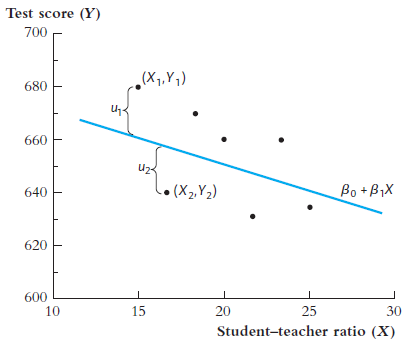
\includegraphics[scale=1.5]{diplomka obrazky/10.png}
    \caption{Znázornenie reziduí.}
    \source{Zdroj: Source of the image.}
\end{figure}

\subsection{Odhad koeficientov modelu lineárnej regresie}

Pri praktických situáciách, ako napríklad určenie dosiahnutých bodov na testoch pomocou počtu žiakov v triedach, je priesečník $\beta_0$ a sklon $\beta_1$ regresnej populačnej priamky neznámy. Teda, potrebujeme dáta, aby sme tieto neznáme koeficienty mohli odhadnúť. 

Povedzme, že chceme porovnať priemernú výšku zárobku mužov a žien, ktorí sú čerstvými absolventmi vysokej školy. Aj napriek tomu, že priemerný zárobok nami vymedzenej ženskej populácie nie je známy (nie je reálne získať dáta o zárobku každej jednej absolventky), môžeme odhadnúť priemer populácie za použitia náhodne vybranej vzorky mužov a žien, ktorí sú čerstvými absolventmi vysokej školy. Prirodzenou štatistikou pre odhad neznámej hodnoty priemerného zárobku absolventiek v populácií, bude napríklad hodnota priemerného zárobku ženských absolventiek v zozbieranej vzorke. Rovnakú logiku uplatníme pri lineárnom regresnom modeli. Nepoznáme hodnotu $\beta_{veľkosť \ triedy}$ populácie, teda sklon neznámej regresnej priamky populácie vzťahujúcej sa ku $X$ (počet žiakov v triede) a $Y$ (dosiahnuté body). Avšak, rovnako ako je možné získať informácie o priemere populácie za použitia vybranej vzorky dát z danej populácie, je taktiež možné dozvedieť sa viac o sklone populačnej regresnej priamky $\beta_{veľkosť \ triedy}$ za použitia vzorky dát. 

\subsection{Metóda najmenších štvorcov}

Model lineárnej regresie v kombinácií s metódou najmenších štvorcov spoločne tvoria jeden zo základných kameňov ekonometrie. Anglický názov predstavuje Ordinary least squares, skrátene OLS. V ďalších častiach textu budeme referovať na Metódu najmenších štvorcov pod skráteným označením OLS.

OLS vyberá koeficienty regresie tak, aby odhadnutá regresná priamka bola čo najbližšie k zozbieraným dátam. To, ako blízko je priamka k dátam, je merané súčtom štvorcov chýb, ktoré sa vyskytli pri odhadovaní $Y$ daný $X$. Teda súčet umocnenej hodnoty, ktorá sa nachádza medzi bodom na odhadnutej priamke, a reálnou nameranou hodnotou zo vzorky.  

Nech $b_0$ a $b_1$ označujú odhady $\beta_0$ a $\beta_1$. Regresná priamka založená na týchto odhadcoch je $b0 + b1X$, teda odhad $Y_i$ odhadnutý za pomoci tejto priamky je $b_0 + b_1X_i$. Chyba, ktorá sa vyskytla pri odhadovaní $í-teho$ pozorovania sa rovná $Y_i - (b_0 + b_1X_i) = Y_i - b_0 - b_1X_i$. Súčet týchto umocnených chýb naprieč všetkými $n$ pozorovaniami je:
\begin{equation}
   \sum_{i=1}^{n}(Y_i - \hat\beta_0 - \hat\beta_1{x}_i)^2 
\end{equation}

Odhad priesečníka a sklonu priamky minimalizáciou súčtu štvorcov chýb, označujeme ako Metódu najmenších štvorcov. Metóda OLS používa na značenie odhadcov $\beta_0$ a $\beta_1$ značenie $\hat\beta_0$ a $\hat\beta_1$. Takto budeme vedieť odlíšiť, či sa jedná o odhadcu, alebo parameter populácie. Teda $\hat\beta_0$ je OLS odhadca $\beta_0$ a $\hat\beta_1$ je OLS odhadca $\beta_1$. Regresná priamka OLS, taktiež nazývaná regresná priamka vzorky\footnote{SRL – Sample regression line.}, je priamka zostrojená za použitia OLS odhacov: 
\begin{equation}
   \hat\beta_0 + \hat\beta_{1}X_i.  
\end{equation}

Odhadnutá hodnota $Y_i$ dané $X_i$, odhadnutá za použitia OLS regresnej priamky, je: 
\begin{equation}
  \hat{Y}_{i} = \hat\beta_0 + \hat\beta_{1}X_i.  
\end{equation}
 
Zvyšok\footnote{Zostatok, rezíduum.} pre $í-té$ pozorovanie predstavuje rozdiel medzi $Y_i$ a jeho odhadnutou hodnotou: 
\begin{equation}
    \hat{u}_i = Y_i - \hat{Y_i}.
\end{equation}

OLS odhadcovia $\hat\beta_0$ a $\hat\beta_1$ sú vypočítaní zo vzorky, a predstavujú ekvivalent koeficientov $\beta_0$ a $\beta_1$ získaných z populácie. Takisto OLS regresná priamka, $\hat\beta_0 + \hat\beta_{1}X_i$, je vzorkovým ekvivalentom populačnej regresnej priamky, $\beta_0 + \beta_{1}X_i$. Zároveň, OLS zostatky, $\hat{u}_i$, sú vzorkovým ekvivalentom populačných náhodných zložiek, $\epsilon_i$. Mohli by sme sa pokúsiť vyrátať OLS odhadcov $\hat\beta_0$ a $\hat\beta_1$ dosadzovaním rôznych hodnôt $b_0$ a $b_1$ opakovane, až kým by sme nenašli tie, ktoré minimalizujú súčet zostatkov v uvedenom modeli. Takáto metóda by však bola veľmi vyčerpávajúca. Predstavíme si vzorce, ktoré sú vyrátané za použitia diferenciálnych a integrálnych počtov. Tieto vzorce sú používané prakticky v každom štatistickom softvéri. Vzorce si nebudeme odvodzovať. Zameriame sa na pochopenie, čo dané vzorce v skutočnosti predstavujú. 

\subsection{Meranie vhodnosti a presnosti predpovede modelu}

Po zostrojení lineárnej regresie sa naskytne otázka:“Ako dobre naša zostrojená regresná priamka vystihuje dáta?“ Je potrebné zamyslieť sa: 
\begin{enumerate}
\item Akú veľkú zásluhu na zmene závislej premennej má regresor?  
\item Sú pozorovania rozmiestnené tesne okolo regresnej priamky, alebo rozptýlené ďaleko od regresnej priamky?
\end{enumerate}
Na zodpovedanie otázok, ako dobre sedí OLS regresná priamka dátam, nám poslúži $R^2$ a štandardná chyba regresie. $R^2$ sa pohybuje v rozsahu medzi 0 a 1, a meria, aká veľká časť zmeny $Y_i$, je vysvetlená zmenou $X_i$. $R^2 = 1$ znamená, že 100\% zmeny $Y_i$ dokážeme vysvetliť pohybom $X_i$. Ak by $Y$ bola cena zmrzliny a $X$ by predstavovalo polevu alebo posýpku, ktorú si na zmrzlinu môžeme pridať, a $R^2$ by malo hodnotu 1, znamenalo by to, že pridanie polevy, ovplyvňuje 100\% zmeny v cene zmrzliny. Teda, jediný faktor ovplyvňujúci cenu zmrzliny, je poleva. Priesečník $\beta_0$ by bol 1€ (základná cena zmrzliny) a $\beta_1$ 0,3€. Pridanie jedného druhu polevy, by navýšilo cenu zmrzliny o 30centov. Každá ďalšia poleva by lineárne zvyšovala cenu o ďalších 30centov. 

Štandardná chyba regresie meria, ako poväčšine vzdialené je $Y_i$ od jej odhadnutej hodnoty, teda bodu na regresnej priamke, ktorý polohou v grafe prislúcha nameranej hodnote.  

\subsection{Koeficient determinácie - $R^2$}

$R^2$ regresie predstavuje časť rozptylu vzorky $Y$, vysvetleného, alebo odhadnutého, prostredníctvom $X$. Pomocou vzorcov na odhadnutú hodnotu $\hat{Y}_{i}$ a zostatkov $\hat{u}_{i}$, môžeme zapísať závislú premennú $Y_i$ ako súčet odhadnutej hodnoty, $\hat{Y}_{i}$, a zostatku $\hat{u}_{i}$ ako: 
\begin{equation}
   {Y}_{i} = \hat{Y}_{i} + \hat{u}_{i}.
\end{equation}
V takomto zápise predstavuje $R^2$ podiel výberového rozptylu $\hat{Y}_{i}$ ku výberovému rozptylu $Y_i$.  
Matematicky môžeme $R^2$ zapísať ako podiel vysvetleného súčtu štvorcov\footnote{SSE - Sum of Squares Explained} a celkového súčtu štvorcov\footnote{SST - Sum of squares Total}. Vysvetlený súčet štvorcov je súčet druhých mocnín odchýlok odhadovanej hodnoty, $\hat{Y}_{i}$, od jej priemeru $\overline{Y}$. Celkový súčet štvorcov je súčet druhých mocnín odchýlok $Y_i$ od jej priemeru $\overline{Y}$: 
\begin{equation}
    SSE = \sum_{i=1}^{n}(\hat{Y}_{i} - \overline{Y})^2
\end{equation}

\begin{equation}
    SST = \sum_{i=1}^{n}({Y}_{i} - \overline{Y})^2
\end{equation}

\begin{figure}[!ht]
    \centering
    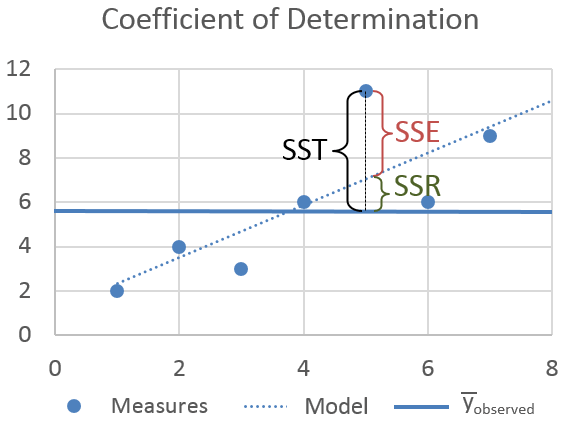
\includegraphics[scale = 0.5]{diplomka obrazky/11.png}
    \caption{Znázornenie častí $R^2$.}
    \source{Zdroj: Source of the image.}
\end{figure}
$R^2$ predstavuje pomer vysvetleného súčtu štvorcov a celkového súčtu štvorcov:
\begin{equation}
    R^2 = \frac{SSE}{SST}
\end{equation}
$R^2$ môžeme zapísať aj ako časť rozptylu $Y_i$, ktorá nie je vysvetlená $X_i$. A to súčtom štvorcov zvyškov z OLS: 
\begin{equation}
    SSR = \sum_{i=1}^{n}\hat{u}_{i}^2
\end{equation}
Z grafu vidíme, že $SST = SSR + SSE$. $R^2$ môžeme vyjadriť aj ako $1$ mínus podiel súčtu štvorcov zostatkov a celkového súčtu štvorcov: 
\begin{equation}
    R^2 = 1 - \frac{SSR}{SST}
\end{equation}
Aj keď $R^2$ vyzerá na prvý pohľad nejednoznačne na pochopenie, a rôzne umocnené súčty sa môžu mýliť, jedná sa jednoducho o korelačný koeficient $r$, umocnený na druhú mocninu. Pri regresii $Y$ na jeden regresor $X$, korelujeme premenné $X$ a $Y$. Ak $\hat\beta_1 = 0$, potom $X_i$ nevysvetľuje žiadnu zmenu $Y_i$, a odhadnutá hodnota $Y_i$ je $\hat{Y}_{i} = \hat\beta_0  = {\overline{Y}}$. V takomto prípade je vysvetlený súčet štvorcov rovný nule, a súčet štvorcov zvyškov sa rovná celkovému súčtu štvorcov, teda $R^2$ je 0. Na rozdiel, ak $X_i$ vysvetľuje všetku zmenu $Y_i$, potom $Y_i = \hat{Y}_{i}$ pre všetky $i$, a všetky zostatky sú rovné nule ($\hat{u}_{i} = 0$), teda $SSE = SST$, teda $R^2$ je v takomto prípade rovné 1. Vo všeobecnosti $R^2$ nenaberá tieto extrémne hodnoty, avšak spadá niekde medzi. $R^2$, ktoré je blízko $1$ naznačuje, že zvolený regresor je dobrý v odhadovaní $Y_i$, naopak $R^2$ blízko 0 naznačuje, že regresor nie je veľmi vhodný v odhadovaní $Y_i$. 

\subsection{Štandardná chyba regresie}

Štandardná chyba regresie\footnote{The Standard Error of the Regression} je odhadca smerodajnej odchýlky náhodnej zložky regresie $u_i$. $u_i$ a $Y_i$ sú vedené v rovnakých jednotkách, keďže $SER$ predstavuje mieru rozptylu pozorovaní okolo regresnej priamky. Napríklad, ak je závislá premenná vedená v eurách, potom $SER$ predstavuje rozsah vychýlenia od regresnej priamky, teda mieru bežnej chyby regresie, a to taktiež v eurách. Avšak náhodná zložka regresie $\epsilon_1, ..., \epsilon_n$ je nepozorovateľná, takže štandardná chyba regresie je vyrátaná za použitia ekvivalentu používaného pri práci s výberom, teda OLS zostatkami $\hat{u}_{1}, ..., \hat{u}_{n}$. Vzorec pre výpočet $SER$ je:
\begin{equation}
    SER = s_{\hat{u}} = \sqrt{s_{\hat{u}}^2}, \ kde \ s_{\hat{u}}^2 = \frac{1}{n-2}\sum_{i=1}^{n}\hat{u}_{i}^2 = \frac{SSR}{n-2},
\end{equation}
kde vzorec pre $s_{\hat{u}}^2$ pracuje s predpokladom, že výberový priemer $OLS$ zostatkov je $0$. Vzorec pre výpočet $SER$ je podobný vzorcu na výpočet výberovej smerodajnej odchýlky $Y$, s tým rozdielom, že $Y_i - \overline{Y}$ je nahradené $\hat{u}_{i}$, a menovateľ sa zmení z $n - 1$ na $n - 2$. Dôvod prečo použijeme $n - 2$ je rovnaký, ako pri použití $n - 1$. Touto úpravou menovateľa predídeme možnej odchýlke výslednej hodnoty. Odčítame $2$, pretože sme regresiou odhadovali dva koeficienty. Jedná sa o korekciu stupňov voľnosti, keďže sme odhadovali dva koeficienty, $\beta_0$  a $\beta_1$, naše dáta prišli o dva stupne voľnosti.  

Rozptyl vzorky $s^2_{Y}$ je:
\begin{equation}
    s^2_{Y} = \frac{1}{n - 1}\sum_{i=1}^{n}(Y_i - \overline{Y})^2.
\end{equation}

\section{Testovanie hypotéz a konfidenčné intervaly}

Tému si vysvetlíme na pokračovaní prípadu o počte žiakov v triede a dosiahnutom počte bodov v teste. Riaditeľ školy si nemyslí, že zmenšovanie počtov žiakov v triedach povedie k lepším výsledkom, a najímanie nových učiteľov považuje za vyhodené peniaze. Ak by sme tento výrok chceli zapísať v jazyku regresnej analýzy, uviedli by sme riaditeľove tvrdenie následovne:"Skutočný kauzálny efekt zmeny počtu žiakov v triede na dosiahnuté skóre je nulový." Teda $\beta_{veľkosť \ triedy} = 0$. 

Potrebujeme riaditeľovi vyvrátiť, že sklon priamky je nulový, čím mu dokážeme, že veľkosť triedy má vplyv na dosahované skóre žiakov. Na vyvrátenie alebo potvrdenie tejto hypotézy použijeme t – test.  

Vo všeobecnosti formulujeme t-štatistiku ako:
\begin{equation}
    t = \frac{estimátor\footnote{Estimátor = odhadca.} - predpoklad \ hypotézy}{štandardná \ chyba \ estimátora}
\end{equation}

\subsection{Obojstranný test sklonu B1}

Testovanie hypotézy o priemernej hodnote populácie za pomoci t-štatistiky:
\begin{equation}
    t = \frac{\overline{Y} - \mu_{0}}{\frac{s_{Y}}{\sqrt{n}}}
\end{equation}

Všeobecný prístup testovania hypotéz o koeficiente $\beta_1$  je rovnaký, ako pri testovaní hypotéz o priemernej hodnote populácie. Kľúčová vlastnosť testovania priemernej hodnoty populácie, na ktorú pri procedúrach spoliehame je, že pri veľkých vzorkách je výberové rozdelenie $\overline{Y}$ približne normálne.  Keďže $\beta_1$ má taktiež normálne výberové rozdelenie pri veľkých vzorkách, hypotézy o skutočnej hodnote sklonu $\beta_1$ môžeme testovať za pomoci totožnej všeobecnej metódy.  

Ako prvé potrebujeme vymedziť hypotézy, ktoré chceme testovať, teda určenie nulovej a alternatívnej hypotézy. V našom prípade je nulovou hypotézou tvrdenie riaditeľa: $\beta_{veľkosť \ triedy} = 0$. Inak povedané, pri nulovej hypotéze skutočný koeficient populácie $\beta_1$  vezme na seba určitú hodnotu, $\beta_{1,0}$\footnote{Nula znamená, že $\beta_1$ naberá hodnotu 0.}. Pri obojstrannom teste, $\beta_1$ nie je rovné $\beta_{1,0}$. Takže nulovú hypotézu a obojstrannú alternatívnu hypotézu zapíšeme ako:
\begin{equation}
    H_{0}:\beta_1 = \beta_{1,0} \ vs. \ H_{1}:\beta_{1} \neq \beta_{1,0}
\end{equation}

Pre otestovanie nulovej hypotézy $H_{0}$ postupujeme takisto, ako pri testovaní populačného priemeru. Postup si zhrnieme do troch krokov. 

\begin{enumerate}
\item Prvým krokom je vyrátanie štandardnej chyby $\hat\beta_1$, teda $SE_{\hat\beta_1}$. Štandardná chyba $\hat\beta_1$ je odhadca $\sigma_{\hat\beta_1}$, čiže smerodajnej odchýlky výberového rozdelenia $\hat\beta_1$. 
Konkrétne:
\begin{equation}
   SE(\hat\beta_{1}) = {\sqrt{\sigma^2_{\hat\beta_{1}}}},  
\end{equation}

kde:
\begin{equation}
  \hat\sigma^2_{\hat\beta_{1}} = \frac{1}{n}\times{\frac{\frac{1}{n - 2}\sum_{i=1}^{n}(X_{i}-\overline{X})^2\hat{u}_{i}^2} {\lbrack{\frac{1}{n}\sum_{i=1}^{n}(X_{i}-\overline{X})^2}\rbrack^2}} . 
\end{equation}

\item Druhým krokom je vyrátanie t-štatistiky:
\begin{equation}
    t = \frac{\hat\beta_{1} - \beta_{1,0}}{SE(\hat\beta_{1})}
\end{equation}

\item

Tretím krokom je vyrátanie $p-hodnoty$, pravdepodobnosti zaznamenania hodnoty $\hat{\beta_{1}}$, ktorá je aspoň tak odlišná od $\beta_{1,0}$, ako nami v skutočnosti vyrátaný odhad $\hat{\beta^{odhadnutá}_{1}}$, za predpokladu, že nulová hypotéza je správna. Zjednodušene povedané, sa jedná o hodnotu pravdepodobnosti, s akou nulová hypotéza $H_0$ môže nastať, respektíve, aká je pravdepodobnosť, že hodnota nulovej hypotézy nastane. Uvedené matematicky:
\begin{equation}
\begin{split}
    p-hodnota & = Pr\footnote{Pravdepodobnosť.}_{H_0}\left[|\hat\beta_{1}-\beta_{1}| > \lvert\hat\beta^{odhadnutá}_{1} - \beta_{1,0}\rvert\right] \\
   & = Pr_{H_0}\left[|\frac{\hat\beta_{1}-\beta_{1,0}}{SE(\hat\beta_{1})}| > |\frac{\hat\beta^{odhadnutá}_{1} - \beta_{1,0}}{SE(\hat\beta_{1})}| \right] \\
   & = Pr_{H_0}(|t| > |t^{odhadnutá}|),
\end{split}    
\end{equation}

\end{enumerate}

kde $Pr_{H_0}$ označuje pravdepodobnosť, vyrátanú v súlade s nulovou hypotézou. Druhá rovnosť pokračuje predelením prvej štandardnou chybou, $SE(\hat\beta_{1})$, nakoniec, $t^{odhadnutá}$ je ozajstne vyrátaná hodnota $t-štatistiky$. Keďže $\hat\beta_{1}$ je zhruba normálne rozdelené pri veľkých vzorkách, podľa nulovej hypotézy je $t-štatistika$ približne rozdelená ako štandardná normálna náhodná premenná, tak pri veľkých vzorkách platí:
\begin{equation}
    p-hodnota = Pr(|Z|>|{t^{odhadnutá}}|) = 2\Phi(-|t^{odhadnutá}|).
\end{equation}

$P-hodnota$ menšia ako $5\%$ nám poskytuje dôkaz proti nulovej hypotéze, v zmysle, že v súlade s nulovou hypotézou je pravdepodobnosť, že dostaneme hodnotu $\hat\beta_{1}$, ktorá je prinajmenšom tak vzdialená od nulovej hypotézy, ako hodnota v skutočnosti pozorovaná, menšia ako $5\%$. Ak je tomu tak, nulová hypotéza je zamietnutá na $5\%$ hladine významnosti.  

Ďalšia možnosť je otestovať hypotézu na $5\%$ hladine významnosti jednoducho, porovnaním absolútnej hodnoty $t-$ ku hodnote $1.96$, čo predstavuje kritickú hodnotu pre obojstranný test, a zamietnutie nulovej hypotézy na $5\%$ hladine významnosti, ak $|t^{odhadnutá}| > 1.96$.

\begin{figure} 
    \centering 
    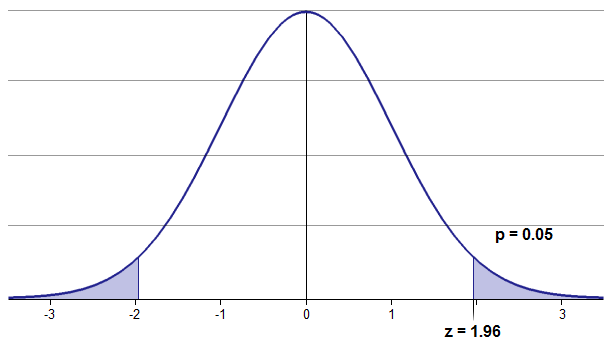
\includegraphics[scale = 0.5]{diplomka obrazky/12.png} 
    \caption{Znázornenie častí $R^2$.} 
    \source{Zdroj: }
\end{figure} 

\subsection{Jednostranné hypotézy o sklone $\beta_{1}$}

Predstavili sme si obojstranné testovanie hypotéz, kde $\beta_{1} = \beta_{1, 0}$ proti hypotéze $\beta_{1} \neq \beta_{1, 0}$. Nazýva sa to obojstranným testom hypotéz preto, pretože alternatívna hypotéza $\beta_{1}$ môže byť buď väčšia, alebo menšia ako $\beta_{1, 0}$. Niekedy sa však hodí viac použiť jednostranný test. V prípade veľkosti tried na výkon študentov si myslíme, že menšie triedy poskytnú študentom kvalitnejšie študijné prostredie, a teda lepšie výkony. V súlade s takouto hypotézou je $\beta_{1}$ negatívna. Ak si to chceme overiť, otestujeme nulovú hypotézu $\beta_{1} = 0$ (žiaden efekt) versus jednostranná alternatíva $\beta_{1} < 0$.  

Pre jednostranný test zapíšeme nulovú a alternatívnu hypotézu ako:  
\begin{equation}
    H_{0}:\beta_{1} = \beta_{1, 0} \ vs. \ \beta_{1} < \beta_{1, 0}, 
\end{equation}
   
kde $\beta_{1, 0}$ je hodnota $\beta_{1}$ podľa nulovej hypotézy (v našom prípade je to $0$, teda veľkosť triedy nemá efekt na výkon študentov), a alternatívna hypotéza $H_1$,  že $\beta_{1}$ je menej ako $\beta_{1, 0}$. Ak by sme chceli alternatívnu hypotézu obrátiť, teda, že $\beta_{1}$ je väčšie ako $\beta_{1, 0}$, nerovnicu jednoducho obrátime.  

Pretože je nulová hypotéza totožná pre jednostranný aj obojstranný test hypotéz, stavba $t-štatistiky$ je rovnaká. Jediným rozdielom medzi jedno a dvojstranným testom hypotéz, je interpretácia $t-štatistiky$. Pri jednostrannom teste je nulová hypotéza zamietnutá proti jednostrannej alternatíve pre veľké negatívne hodnoty, avšak nie pre veľké pozitívne hodnoty $t-štatistiky$. Namiesto zamietnutia pri $|t^{odhadnutá}| > 1.96$, je hypotéza zamietnutá na 5\% hladine významnosti ak $|t^{odhadnutá}| < -1.64$. $t-hodnota$ sa mení preto, pretože neodkusneme 2.5\% z každej strany, ale 5\% z jednej. Tým pádom sa zväčší chvostík rozdelenia, a zmenší sa jadro z 1.96 smerodajných odchýlok na 1.64.  

$p-hodnota$ pre jednostranný test hypotéz je získaná z kumulatívneho štandardného normálneho rozdelenia ako:
\begin{equation}
    p-hodnota = Pr(Z<t^{odhadnutá})=\Phi(t^{odhadnutá}).\footnote{Jednostranný, ľavostranný test.}
\end{equation}

Ak je alternatívnou hypotézou, že $\beta_{1}$ je väčšie ako $\beta_{1, 0}$, nerovnosť v nerovnici sa obráti, takže $p-hodnota$ je pravdepodobnosť pravého chvosta, $Pr(Z>t^{odhadnutá})$. Teda pravdepodobnosť, s akou sa hodnoty v priemere objavia v pravom chvoste rozdelenia.  

\subsection{Testovanie hypotéz o priesečníku $\beta_{0}$}

Nulová hypotéza týkajúca sa priesečníka, a jej obojstrannú alternatívnu hypotézu zapíšeme ako:
\begin{equation}
    H_{0}:\beta_{0} = \beta_{0, 0} \ vs. \ \beta_{0} < \beta_{0, 0}.
\end{equation}

Postup ostáva, ako pri testovaní sklonu. Platí to aj pri jednostrannom teste.

Testovanie hypotéz je užitočné v prípade, keď zmýšľame o konkrétnej nulovej hypotéze. Byť schopný zamietnuť, alebo nezamietnuť našu hypotézu na základe štatistickej inferencie, predstavuje silný štatistický nástroj, pri vysporiadaní sa s pochybnosťami, a pri zisťovaním informácií o populácií zo vzorky. Často sa však stáva, že žiadna konkrétna hypotéza o regresnom koeficiente nie je dominantná. V takomto prípade by sme uvítali rozmedzie hodnôt koeficientu, ktoré sú konzistentné s dátami. S týmto nám pomôžu konfidenčné intervaly (intervaly spoľahlivosti). 

\section{Intervaly spoľahlivosti pre regresné koeficienty}

Keďže akýkoľvek štatistický odhad sklonu $\beta_{1}$, sa nevyhnutne spája s neistotou spôsobenou výberom, nemôžeme presne určiť skutočnú hodnotu $\beta_{1}$ za použitia vzorky dát. Môžeme však používať $OLS$ odhadcov, a ich štandardné chyby, na skonštruovanie intervalov spoľahlivosti pre sklon $\beta_{1}$, alebo pre priesečník $\beta_{0}$. 

\subsection{Interval spoľahlivosti pre $\beta_{1}$}

95\% konfidenčný interval pre $\beta_{1}$ má dve rovnocenné definície. Prvá tvrdí, že konfidenčný interval je súbor hodnôt, ktoré nemôžu byť zamietnuté pri použití obojstranného testu hypotéz s 5\% hladinou významnosti. Druhá tvrdí, že konfidenčný interval je interval, ktorý má 95\% pravdepodobnosť, že bude obsahovať skutočnú hodnotu $\beta_{1}$. Inak povedané, ak by sme zozbierali nekonečné množstvo vzoriek a z každej zostavili konfidenčný interval, 95\% z nich by obsahovalo skutočnú hodnotu $\beta_{1}$. Pretože tento interval obsahuje skutočnú hodnotu v 95\% všetkých vzoriek, vravíme, že máme 95\% úroveň spoľahlivosti.

Dôvod prečo sú tieto dve definície rovnocenné je nasledovný. Test hypotéz s hladinou významnosti 5\% zamietne, podľa definície, skutočnú hodnotu $\beta_{1}$ iba v 5\% prípadoch všetkých možných vzoriek. Teda v 95\% všetkých možných vzoriek skutočná hodnota nebude zamietnutá. Nakoľko 95\% interval spoľahlivosti je súborom všetkých hodnôt $\beta_{1}$, ktoré nie sú zamietnuté na 5\% hladine spoľahlivosti, skutočná hodnota $\beta_{1}$ bude obsiahnutá v intervale spoľahlivosti v 95\% všetkých možných vzoriek.

V princípe, 95\% interval spoľahlivosti môže byť vyrátaný testovaním všetkých možných hodnôt B1 (teda testovaním nulovej hypotézy $\beta_{1} = \beta_{1, 0}$ pre všetky hodnoty $\beta_{1, 0}$) na 5\% hladine spoľahlivosti za použitia t-štatistiky. 95\% konfidenčný interval je v takomto prípade súbor všetkých hodnôt $\beta_{1}$, ktoré nie sú zamietnuté. Zostrojenie t-štatistiky pre všetky hodnoty $\beta_{1}$ by však zabralo nekonečne veľa času. 
Jednoduchší spôsob zostrojenia intervalu spoľahlivosti sa naskytne, keď si uvedomíme, že t-štatistika odmietne vyslovenú hodnotu hypotézu $\beta_{1, 0}$ v prípade, keď je $\beta_{1, 0}$ mimo intervalu $\hat\beta_{1} \pm 1.96SE(\hat\beta_{1})$. To znamená, že 95\% konfidenčný interval pre $\hat\beta_{1}$ je interval: 
\begin{equation}
    [\hat\beta_{1} - 1.96SE(\hat\beta_{1}) \ , \ \hat\beta_{1} + 1.96SE(\hat\beta_{1})].
\end{equation}

\subsection{Interval spoľahlivosti pre $\beta_0$}

95\% konfidenčný interval pre $\beta_0$ zostrojíme rovnako ako pri $\beta_1$. Namiesto $\hat\beta_1$  použijeme $\hat\beta_0$  a namiesto $SE(\hat\beta_{1})$ zas $SE(\hat\beta_{0})$.

$OLS$ regresia výšky dosiahnutého hodnotenia na veľkosť tried poskytla hodnoty odhadcov $\hat\beta_{1} = -2.28$ a $SE(\hat\beta_{1}) = 0.52$. Obojstranný 95\% interval spoľahlivosti pre $\hat\beta_{1}$ je $\{-2.28 \pm 1.96 \times 0.52\}$, alebo $\{-3.30 \leq \beta_{1} \leq -1.26\}$. Hodnota $\beta_{1} = 0$ nie je obsiahnutá v intervale spoľahlivosti, takže nulová hypotéza $\beta_{1} = 0$ môže byť zamietnutá na hladine spoľahlivosti 5\%. 

\subsection{Interval spoľahlivosti pre predpovedaný efekt zmeny $X$}

Konfidenčný interval pre $\beta_1$ môže byť použitý na zostrojenie 95\% intervalu spoľahlivosti pre predpovedaný efektu všeobecnej zmeny v $X$. Uvažujme so zmenou $X$ v určitej miere $\Delta x$. Očakávaná zmena v $Y$ spojená so zmenou v $X$ je $\beta_{1} \Delta x$. Sklon populácie $\beta_1$ nie je známy, avšak keďže môžeme skonštruovať konfidenčný interval pre $\beta_1$, môžeme taktiež zostrojiť konfidenčný interval pre očakávaný efekt $\beta_{1} \Delta x$. Nakoľko jeden koniec 95 intervalu spoľahlivosti pre $\beta_1$ je $\hat\beta_{1} - 1.96SE(\hat\beta_{1})$, a predpovedaný následok zmeny $\Delta x$ za použitia odhadu pre $\beta_1$ je $[\hat\beta_{1} - 1.96SE(\hat\beta_{1})] \times \Delta x$. Druhý koniec intervalu spoľahlivosti je $\hat\beta_{1} + 1.96SE(\hat\beta_{1})$, a predpovedaný efekt zmeny za použitia odhadu je $[\hat\beta_{1} + 1.96SE(\hat\beta_{1})] \times \Delta x$. Teda 95\% interval spoľahlivosti pre dôsledok zmeny $X$ v miere $\Delta x$ môžeme vyjadriť ako 95\% konfidenčný interval pre $\beta_{1} \Delta x$:
\begin{equation}
   [\hat\beta_{1} - 1.96SE(\hat\beta_{1})\Delta x \ , \ \hat\beta_{1} + 1.96SE(\hat\beta_{1})\Delta x]. 
\end{equation}
Uveďme si príklad. Ak by sme chceli zmeniť pomer študentov k učiteľom (vyjadrenie veľkosti tried) o 2 jednotky, tak keďže $95\%$ interval spoľahlivosti pre $\beta_1$ je $[-3.30, -1.26]$, dôsledok zníženia pomeru o 2 jednotky by mohol mať dopad až $-3.30 \times (-2) = 6.6$ bodu, alebo len $-1.26 \times (-2) = 2.52$. Takže zníženie pomeru študentov k učiteľom o hodnotu 2 by malo odhadovaný efekt navýšenia bodovej úspešnosti študentov v testoch medzi 2.52 a 6.6 bodov, s 95\% úrovňou spoľahlivosti. Ak je pomer študentov k učiteľom $10:1$, tak na jedného učiteľa pripadá $10$ žiakov. Zníženie z 10 na 8 študentov na jedného učiteľa by malo predpovedaný efekt vyrátaný vyššie. 

\section{Heteroskedasticita a Homoskedasticita}

Náhodná zložka ${u}_{i}$  je homoskedastická, ak rozptyl podmieneného rozdelenia ${u}_{i}$ daný\footnote{(${u}_{i}$ | $X_{i}$)} $X_{i}$, je konštantný pre $i = 1, ..., n$, a obzvlášť nezávisí na $X_{i}$. Ak táto podmienka nie je splnená, hovoríme, že náhodná zložka je heteroskedastická. Najlepšie to vysvetlíme ilustráciou náhodných zložiek a porovnaním ich rozptylov vizuálne. Distribúcia náhodnej zložky ${u}_{i}$ je ilustrovaná pre viaceré hodnoty $x$. Keďže sa toto rozdelenie týka konkrétne vyznačených hodnôt $x$, jedná sa o podmienené rozdelenie ${u}_{i}$ daný $X_{i} = x$, ktoré má podľa prvej podmienky najmenších štvorcov priemer rovný nule pre všetky $x$. Na prvom grafe majú všetky tieto podmienené rozdelenia rovnaký rozptyl, inak povedané, rozptyl všetkých týchto rozdelení je rovnaký pre rôzne hodnoty $x$. Podmienená zmena ${u}_{i}$ daný $X_{i} = x$, nezávisí od $x$, teda neznáme zložky sú homoskedastické. 

Na druhej strane, druhý graf zobrazuje prípad, kedy sa podmienené rozdelenie ${u}_{i}$ rozpína s narastajúcim $x$. Pri malých hodnotách $x$ je rozdelenie úzke, avšak pri väčších hodnotách $x$ je rozdelenie širšie. V druhom grafe rozptyl ${u}_{i}$ daný $X_{i} = x$ narastá s $x$, teda neznáma zložka je heteroskedastická. 
\begin{figure}[!ht] 
    \centering 
    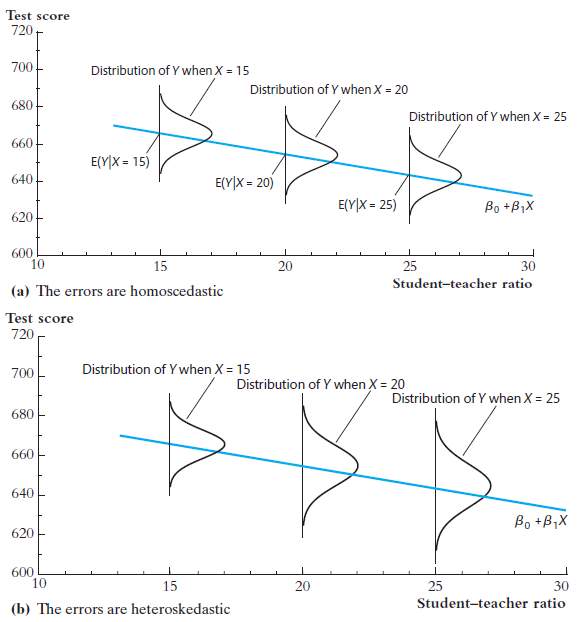
\includegraphics[scale = 1.25]{diplomka obrazky/13.png} 
    \caption{a) Homoskedasticita. b) Heteroskedasticita.} 
    \source{Zdroj: Source of the image.} 
\end{figure} 

Pretože metóda najmenších štvorcov nemá medzi svojimi predpokladmi žiadne vymedzené obmedzenia týkajúce sa podmieneného rozptylu, predpoklad platí aj v prípade homoskedasticity aj heteroskedasticity. Z toho dôvodu $OLS$ odhadcovia ostanú nestranní, konzistentní a asymptoticky normálni, či už je neznáma zložka heteroskedastická, alebo homoskedastická. Existujú vzorce na výpočet odchýlky, ktoré vopred rátajú, že neznáma zložka je homoskedastická. Z historických dôvodov sú často vzorce tohto typu prednastavené v štatistickom softvéri. Ak je náhodná zložka heteroskedastická, tieto vzorce nie je vhodné použiť. Napríklad, vyrátaná t-štatistika nebude mať štandardné normálne rozdelenie, ani pri veľkých vzorkách. Na druhú stranu, keďže homoskedasticita je mimoriadny prípad heteroskedasticity, odhadcovia $\hat\sigma^2_{\hat\beta_{1}}$ a $\hat\sigma^2_{\hat\beta_{0}}$ rozptylu $\hat\beta_{1}$ a $\hat\beta_{0}$ ponúknu platný štatistický úsudok, či už je neznáma zložka heteroskedastická, alebo homoskedastická. Tým pádom sú testy hypotéz a intervaly spoľahlivosti založené na týchto štandardných chybách platné, či už sú náhodné zložky heteroskedastické, alebo nie. Takéto štandardné chyby sa nazývajú heteroskedasticky-robustné. Ak sú štandardné chyby za použitia vzorcov aj pre homoskedasticitu aj heteroskedastickú robustnosť rovnaké, nič sa nestane, ak použijeme heteroskedasticky-robustné štandardné chyby. Ak sa líšia, mali by sme použiť výsledok z heteroskedasticky-robustného výpočtu. Najjednoduchší spôsob je takéto heteroskedasticky-robustné vzorce pre výpočet štandardnej chyby používať stále. 

\section{Lineárna regresia s viacnásobným regresorom}

Aj napriek tomu, že školy s menším podielom študentov k učiteľom majú tendenciu mať lepšie výsledky v testoch, skutočnosť je pravdepodobne taká, že okrem počtu žiakov v triedach vplýva na výšku dosiahnutých bodov aj niečo iné. Cieľom viacnásobnej lineárnej regresie, je práve vyhnutie sa odchýlke, ktorá môže byť spôsobená vynechaním vplyvných faktorov, ich  nezakomponovaním do lineárnej regresie. Vynechané premenné, ako napríklad vlastnosti študentov, môžu spôsobiť, že $OLS$ odhadca odhadne skreslené hodnoty koeficientov, teda $OLS$ odhadca bude neobjektívny, skreslený. Hlavnou myšlienkou viacnásobnej lineárnej regresie je, že ak máme dáta o týchto vynechaných premenných, môžeme ich zahrnúť do lineárnej regresie ako ďalší regresor, a takto odhadnúť kauzálny efekt jedného regresora (pomer študentov k učiteľom) , zatiaľ čo ostatné premenné zachováme konštantné (vlastnosti študentov). 

Alternatívne, ak nás viac zaujíma predikcia než kauzálna inferencia, model viacnásobnej regresie nám umožňuje použiť viacero premenných ako regresory, t.j. viacero prediktorov, na vylepšenie predikcií vytvorených jedným regresorom jednoduchou lineárnou regresiou.

\subsection{Odchýlka spôsobená vynechanou premennou}

Ak je regresor (pomer študentov k učiteľom) korelovaný s nezávislou premennou (vlastnosti študentov), ktorú sme do modelu nezahrnuli, avšak ovplyvňuje závislú premennú modelu, bude $OLS$ odhadca trpieť odchýlkou vynechanej premennej. 
Odchýlka vynechanej premennej nastane, ak sú splnené dve podmienky:
\begin{enumerate}
\item opomenutá premenná je korelovaná s regresorom (nezávislou premennou), ktorý je zahrnutý v modeli,
\item opomenutá premenná má súvis a vplyv na závislú premenú.
\end{enumerate}
Platnosť podmienok si osvetlíme na nasledujúcich príkladoch:
\begin{enumerate}
\item Za vynechanú premennú považujeme vlastnosť študentov, konkrétne ich jazykové znalosti, merané tým, či školy do ktorých chodia, vyučujú v ich materinskom jazyku, alebo nie. Jazykové znalosti, a pomer študentov k učiteľom sú korelované (školy pre prisťahované deti zvyknú mať väčší počet detí na jedného učiteľa). Tým je prvá podmienka odchýlky vynechanej premennej splnená. Je pochopiteľné, že študenti, ktorí v jazyku používanom na škole nie sú na úrovni domácich, budú mať ťažšie podmienky pri písaní testov, a teda očakávame aj horšie výsledky. Čím spĺňame aj druhú podmienku. Takto by sme teda vynechaním tejto premennej v modeli zapríčinili, že by $OLS$ odhadca nesprávne premietol dáta do koeficientov odhadcov.
\item Ďalšou vynechanou premennou je čas dňa, kedy študenti tento štandardizovaný test, na ktorom je postavený náš súbor dát, písali. Ak sa čas písania testu líši medzi rôznymi mestskými časťami kvôli dôvodu, ktorý nie je spojený s počtom žiakov v triede, potom prvá podmienka nie je splnená. Avšak čas písania testu môže ovplyvňovať výšku dosiahnutého hodnotenia v teste (bdelosť študentov nie je počas celého dňa rovnaká), tým pádom, premenná spĺňa druhú podmienku. Nuž, keďže v tomto prípade čas písania testu nie je korelovaný s počtom žiakov na učiteľa, táto premenná (pomer študentov k učiteľom) nemôže chybne zachytiť efekt vynechanej premennej (fáza dňa, kedy bol test absolvovaný), na zmenu závislej premennej (dosiahnuté skóre). Čo znamená, že nezahrnutie premennej o fáze dňa, kedy bol test písaný, nebude mať za následok odchýlku vynechanej premennej. 
\item Ďalšia vynechaná premenná predstavuje počet parkovacích miest pre učiteľov na študenta. Táto premenná spĺňa prvú podmienku, ale druhú nie. Školy s viacerými učiteľmi na žiaka, majú pravdepodobne viac parkovacích miest pre učiteľov, čo zaručuje splnenie prvej podmienky. Avšak, vyučovanie prebieha vo vnútorných priestoroch školy, a nie na parkovisku. Čiže parkovacie miesta nemajú žiaden priamy efekt na vyučovanie, čo odporuje splneniu druhej podmienky. Pretože parkovacie miesta na žiaka nemajú vplyv na výšku skóre, vynechanie tejto premennej z modelu nepovedie k odchýlke vynechanej premennej.
\end{enumerate}

Prítomnosť odchýlky opomenutej premennej znamená, že predpoklad najmenších štvorcov pre kauzálnu inferenciu $E(u_{i} | X_{i}) = 0$, nie je splnený. Aby sme pochopili prečo, pripomeňme si, že náhodná zložka $u_i$ v modeli jednoduchej lineárnej regresie reprezentuje všetky faktory, iné ako $X_{i}$, ktoré majú vplyv na $Y_{i}$. Ak nejaký z týchto iných faktorov je korelovaný s $X_{i}$, znamená to, že náhodná zložka (ktorá obsahuje tento faktor) je korelovaná s $X_{i}$. Inak povedané, ak má opomenutá premenná vplyv na $Y_{i}$, tento vplyv je zahrnutý v náhodnej zložke, a ak je táto opomenutá premenná korelovaná s $X_{i}$, potom je náhodná zložka korelovaná s $X_{i}$. Pretože $u_{i}$ a $X_{i}$ sú korelované, podmienený priemer (očakávaná hodnota) $u_{i}$ daný $X_{i}$ je nenulový. Táto korelácia porušuje prvú podmienku metódy najmenších štvorcov, čoho dôsledkom je odchýlka $OLS$ odhadcu. Táto odchýlka nezmizne ani pri veľkých vzorkách, čo robí $OLS$ odhadcu nekonzistentným. 

\subsubsection{Vzorec pre odchýlku vynechanej premennej}

Označme koreláciu medzi $X_{i}$ a $u_{i}$ ako $corr(X_{i}, u_{i}) = \rho_{Xu}$. Predpokladajme, že druhá a tretia podmienka najmenších štvorcov platí, avšak prvá nie, pretože $\rho_{Xu}$ je nenulové. $OLS$ odhadca má limitu:
\begin{equation}
    \hat\beta_{1}\xrightarrow[\text{}]{\text{\; p \; }}\beta_{1}+\rho_{Xu}\frac{\sigma_{u}}{\sigma_{X}}.
\end{equation}

Ak veľkosť vzorky rastie, $\hat\beta_{1}$ je bližšie k $\beta_{1} + \rho_{Xu}(\sigma_{u} / \sigma_{X})$ s narastajúcou pravdepodobnosťou. 
\begin{enumerate}
\item  Odchýlka opomenutej premennej je problém, či už je vzorka malá alebo veľká, pretože $\hat\beta_{1}$  nekonverguje s pravdepodobnosťou k skutočnej hodnote $\beta_{1}$. $\hat\beta_{1}$ má odchýlku, a je nekonzistentný, čo znamená, že $\hat\beta_{1}$ je nekonzistentným odhadcom $\beta_{1}$, za prítomnosti odchýlky opomenutej premennej. Časť vzorca $\rho_{Xu}(\sigma_{u} / \sigma_{X})$ predstavuje odchýlku v $\hat\beta_{1}$, ktorá pretrvá aj pri veľkých vzorkách.  
\item Veľkosť odchýlky závisí od absolútnej výšky korelácie regresora, a náhodnej zložky. 
\item Smer odchýlky závisí na $pozitivite / negativite$ korelácie medzi $X$ a $u$.
\end{enumerate}
Náhodné kontrolované experimenty\footnote{RCT - Randomized contorlled trials.} napomáhajú odstraňovaniu veľkého množstva týchto odchýlok.

\subsection{Model viacnásobnej lineárnej regresie}

Model viacnásobnej lineárnej regresie rozširuje model jednoduchej lineárnej regresie o dodatočné regresory. Pri použití modelu pre kauzálnu inferenciu nám model s viacerými regresormi umožňuje odhadnúť efekt na $Y_{i}$ pri úprave jednej premennej ($X_{1i}$), pričom ostatné premenné ($X_{2i}$, $X_{3i}$, atď) ostanú konštantné. Pri príklade o výške dosiahnutých bodov študentov a počtu učiteľov na žiaka nám umožní model viacnásobnej lineárnej regresie izolovať efekt počtu učiteľov na žiaka ($X_{1i}$) na výšku skóre ($Y_{i}$), pričom premenná $X_{2i}$, ktorá znázorňuje pomer žiakov, ktorí neštudujú v materinskom jazyku, ostane napriek zmene (v $X_{1i}$) konštantná. Pri použití modelu pre predikciu, použitie viacerých regresorov môže vylepšiť predikcie. 

\subsubsection{Regresná priamka populácie}

Uvažujme s dvoma nezávislými premennými $X_{1i}$ a $X_{2i}$. V modeli viacnásobnej lineárnej regresie je priemerný vzťah medzi týmito dvoma nezávislými premennými a závislou premennou $Y$ vyjadrený lineárnou funkciou:
\begin{equation}
    E(Y_{i} | X_{1i} = x_{1},X_{2i}=x_{2}) = \beta_{0} + \beta_{1}x_{1} + \beta_{2}x_{2},
\end{equation}
kde $E(Y_{i} \ daný \ X_{1i} = x_{1},X_{2i}=x_{2})$ je podmienená očakávaná hodnota $Yi$ daný, že $X_{1i} = x_{1},X_{2i}=x_{2}$. 
Takáto lineárna funkcia sa v modeli viacnásobnej lineárnej regresie nazýva populačná regresná priamka, alebo populačná regresná funkcia. Je to vzťah, ktorý priemerne platí v populácií pre $Y$ a všetky regresory $X_k$. Koeficient $\beta_{0}$ je priesečník, koeficient $\beta_{1}$ je koeficient sklonu $X_{1i}$ a koeficient $\beta_{2}$ je koeficient sklonu $X_{2i}$. Interpretácia koeficientu $\beta_{1}$ v modeli viacnásobnej lineárnej regresie populácie sa líši od jednoduchej lineárnej regresie, kde $X_{1i}$ bol jediným regresorom. V uvedenom modeli je $\beta_{1}$ odhadnutá zmena $Y$ medzi dvoma pozorovaniami, pri zmene $X_1$ o jednu jednotku, pričom $X_2$ ostáva konštantné. Táto interpretácia $\beta_{1}$ vyplýva z porovnávania odhadov dvoch pozorovaní s rovnakou hodnotou $X_2$, avšak dvoma hodnotami $X_1$, ktoré sa líšia o $\Delta X_{1}$. Tým pádom prvé pozorovanie pracuje s hodnotami $X$ ($X1$ a $X2$), a druhé pozorovanie s hodnotami $X$ ($X_{1} + \Delta X_{1}, X_{2}$). Odhadovaná hodnota $Y$ pre prvé pozorovanie je daná rovnicou:
\begin{equation}
    Y = \beta_{0} + \beta_{1} X_{1} + \beta_{2} X_{2}.
\end{equation}

Odhadovaná hodnota $Y$ pre druhé pozorovanie je $Y + \Delta Y$, pre ktorú:
\begin{equation}
    Y + \Delta Y = \beta_{0} + \beta_{1} (X_{1} + \Delta X_{1}) + \beta_{2} X_{2}.
\end{equation}
Rovnicu pre $\Delta Y$ pokiaľ ide o $\Delta X_{1}$ dostaneme odčítaním rovnice $Y = \beta_{0} + \beta_{1} X_{1} + \beta_{2} X_{2}$ od $Y + \Delta Y = \beta_{0} + \beta_{1} (X_{1} + \Delta X_{1}) + \beta_{2} X_{2}$, výsledkom čoho je $\Delta Y = \beta_{1}\Delta X_{1}$, čo môžeme prepísať ako:
\begin{equation}
    \beta_{1} = \frac{\Delta Y}{\Delta X_{1}},
\end{equation}
pričom udržiavame $X_2$ konštantné.

Koeficient $\beta_{1}$ je teda rozdiel v odhadnutej hodnote $Y$ (rozdiel podmienených očakávaní $Y$) medzi dvomi pozorovaniami pri jednotkovej zmene v $X_1$, pričom držíme $X_2$ konštantné. $\beta_{1}$ predstavuje čiastkový efekt $X$ na $Y$, držiac $\beta_{1}$ nemenné. Interpretácia $\beta_{0}$ je rovnaká ako pre jednoduchú lineárnu regresiu.  
Všeobecný model pre viacnásobnú regresiu je:
\begin{equation}
    Y_{i} = \beta_{0} + \beta_{1} X_{1i} + \beta_{1} X_{2i} + ... + \beta_{k} X_{ki} + \epsilon_{i}, \ i = 1, ..., n,
\end{equation}
kde:
\begin{itemize}
\item  $Y_i$ je $í-te$ pozorovanie závislej premennej $X_{1i}, X_{2i}, ..., X_{ki}$ sú $í-te$ pozorovania každého z $k$ regresorov, a $\epsilon_i$ je náhodná zložka.
\item Názvoslovie $OLS$ pre viacnásobný model lineárnej regresie je rovnaké ako pre model jednoduchej lineárnej regresie. 
\end{itemize}

Definícia homoskedasticity a heteroskedasticity v modeli viacnásobnej regresie je obšírnejšia v porovnaní s definíciou pre model jednoduchej regresie. Náhodná zložka $\epsilon_{i}$ v modeli viacnásobnej regresie je homoskedastická, ak rozptyl podmieneného rozdelenia $\epsilon_{i}$ daný $X_{1i}, ..., X_{ki}, var(u_{i}|X_{1i}, ..., X_{ki})$, je konštantný pre $i = 1, ..., n$, čím nie je závislý na hodnotách $X_{1i}, ..., X_{ki}$. Ak táto podmienka nie je splnená, náhodná zložka je heteroskedastická.

\subsection{Meranie vhodnosti modelu vo viacnásobnej regresii}

\subsubsection{Štandardná chyba regresie}

Vo viacnásobnej regresii je štandardná chyba regresie vyrátaná ako:
\begin{equation}
    SER = s_{\hat{u}} = \sqrt{s_{\hat{u}}^2},  \ kde \  s_{\hat{u}}^2 =\frac{1}{n-k-1}\sum_{i=1}^{n}\hat{u_{i}}^2 = \frac{SSR}{n-k-1}.
\end{equation}

Jediným rozdielom medzi definíciou štandardnej chyby regresie vo viacnásobnej a jednoduchej regresií je iný menovateľ. V definícií pre viacnásobnú regresiu je to $n - k - 1$, namiesto $n - 2$. Menovateľ $n - 2$ pri regrersii s jedným regresorom upravuje odhadcu kvôli nadol smerujúcej odchýlke, ktorá vzniká pri odhade dvoch koeficientov, priesečníku a sklonu. Vo vzorci pre viacnásobnú regresiu menovateľ $n - k - 1$ upravuje pre nadol smerujúcu odchýlku, ktorá vzniká pri odhade $k + 1$ koeficientov. Takisto ako pri už skôr uvedenom vzorci pre jednoduchú regresiu, použitie $n - k - 1$ namiesto $n$ sa nazýva úprava stupňov voľnosti. Pri jednom regresore sa $k = 1$, teda vzorec pre odhad štandardnej chyby regresie pre jednoduchú a viacnásobnú regresiu bude zhodný. Pri veľkom $n$ je efekt úpravy stupňov voľnosti zanedbateľný.   

\subsubsection{Koeficient determinácie - $R^2$}











% !TeX encoding = UTF-8
% !TeX spellcheck = sk_SK
% !TeX root=tukedip.tex
\section{Jadro práce}

Začnime rovnicou

\begin{equation}\label{r:2}
\frac{\ud^2y}{\ud t^2}+\frac{\ud y}{\ud t}+y =0, \qquad y(0)=1, \quad
y\,'(0)=15.
\end{equation}

Grafický priebeh riešenia tejto rovnice vidíme na Obrázku \ref{o:2}.

\begin{figure}[ht!]
\centering
\includegraphics[width=.95\textwidth,angle=0]{relaxcas.pdf}
\caption{Teplotná závislosť spinovo-mriežkového relaxačného
času}\label{o:3}
\end{figure}

%\tabcolsep=3pt % sirka stlpcov
%\renewcommand{\arraystretch}{1.2} % riadkovanie
\begin{table}[ht!]
\centering
\caption{Parametre získané z~meraní spinovo-mriežkových relaxačných
časov $T_1$}\label{t:2}
\medskip
\newcolumntype{d}{D{,}{,}{-1}}
\begin{tabular}{||c||d|d|d|d|d||}
\hhline{|t:==t:==:==:t|}
\multicolumn{1}{||c||}{}&\multicolumn{1}{c|}{PP --
01}&\multicolumn{1}{c|}{PP -- 05}&\multicolumn{1}{c|}{PP --
10}&\multicolumn{1}{c|}{PP -- 16}&\multicolumn{1}{c||}{PP -- 22} \\
\hhline{|:==:==:==:|}
C $\cdot 10^8$~(s$^{-2}$) & 10,1 & 10,0 & 11,0 & 9,2 & 8  \\
\hhline{||-|-|-|-|-|-||}
$\tau_0 \cdot 10^{-14}$~(s) & 2,63 & 1,44 & 0,95 & 2,21 & 10,83  \\
\hhline{||-|-|-|-|-|-||}
$E_{\text a}$~(kJ) & 34,26 & 8,33 & 39,76 & 37,31 & 31,86  \\
\hhline{||-|-|-|-|-|-||}
$T_{\min}$~(K) & 354 & 367 & 367 & 369 & 367  \\
\hhline{||-|-|-|-|-|-||}
$T_{1\min}$~(ms) & 141 & 160 & 157 & 175 & 181  \\
\hhline{||-|-|-|-|-|-||}
$\Delta M_2$~(Gs$^2$) & 5,49 & 5,66 & 5,16 & 5,09 & 5,02  \\
\hhline{|b:==b:==:==:b|}
\end{tabular}
\end{table}


%
\section{Z\'aver (zhodnotenie rie\v{s}enia)}

Táto časť\/ záverečnej práce je povinná. Autor uvedie zhodnotenie
riešenia. Uvedie výhody, nevýhody riešenia,  použitie výsledkov, ďalšie
možnosti a~pod., prípadne načrtne iný spôsob riešenia úloh, resp.
uvedie, prečo postupoval uvedeným spôsobom.
%
% !TeX encoding = UTF-8
% !TeX spellcheck = sk_SK
% !TeX root=tukedip.tex
%%
\begin{thebibliography}{19}
\addcontentsline{toc}{section}{\numberline{}Zoznam použitej
literatúry}

\harvarditem{Barančok et al.}{1995}{barancok}
BARANČOK, D. et al. 1995. \emph{The effect of semiconductor surface
treatment on LB film/Si interface.} In:~Physica Status Solidi (a), 
ISSN 0031-8965, 1995, vol. 108, no.~2, \mbox{pp. K~87--90}

\harvarditem{Benčo}{2001}{benco}
BENČO, J. 2001. \emph{Metodológia vedeckého výskumu.} Bratislava~:
IRIS, 2001, ISBN 80\discretionary{-}{-}{-}89018-27-0

\harvarditem{Gonda}{2001}{gonda}
GONDA, V. 2001. \emph{Ako napísať a~úspešne obhájiť diplomovú prácu.}
Bratislava~: Elita, 2001, 3. doplnené a~prepracované vydanie, 120~s.
ISBN 80-8044-075-1

\harvarditem{Jadr. fyz. a~tech.}{1985}{slovnik}
\emph{Jadrová fyzika a~technika: Terminologický výkladový slovník.}
2.~rev.~vyd. Bratislava~: ALFA, 1985. 235~s. ISBN 80-8256-030-5

\harvarditem{Katuščák}{1998}{kat}
KATUŠČÁK, D. 1998. \emph{Ako písať vysokoškolské a~kvalifikačné
práce.} Bratislava~: Stimul, 1998, 2.~doplnené vydanie. 121~s. ISBN
80-85697-82-3

\harvarditem{Lamoš a~Potocký}{1989}{lamos}
LAMOŠ, F. -- POTOCKÝ, R. 1989. \emph{Pravdepodobnosť a~matematická
štatistika.} 1.~vyd. Bratislava~: Alfa, 1989. 344~s. ISBN 80-8046-020-5

\harvarditem{Sýkora a~i.}{1980}{sykora}
SÝKORA, F. a~iní. 1980. \emph{Telesná výchova a~šport.} 1.vyd.
Bratislava~: SPN, 1980. 35~s. ISBN 80-8046-020-5

\harvarditem{Steinerová}{2000}{steinerova}
STEINEROVÁ, J. 2000. \emph{Základy filozofie človeka v~knižničnej
a~informačnej vede.} In:~Kimlička, Š., Knižničná a~informačná veda na
prahu informačnej spoločnosti. Bratislava~: Stimul, 2000. ISBN
80-2274-035-2, s. 327--334

\harvarditem{Šumichrast}{1995}{sumichrast}
ŠUMICHRAST, Ľ. 1995. \emph{On the performance of higher approximations
of radiation boundary conditions for the simulation of wave propagation
in structures of integrated optics.} In:~Photonics '95. Prague~: CTU,
1995, pp. 159--161

\harvarditem{Šumichrast}{1995}{sumichras}
ŠUMICHRAST, Ľ. 1995. \emph{On the performance of higher approximations
	of radiation boundary conditions for the simulation of wave propagation
	in structures of integrated optics.} In:~Photonics '95. Prague~: CTU,
1995, pp. 159--161

\end{thebibliography}
%
\section*{Zoznam pr\'iloh}
\addcontentsline{toc}{section}{\numberline{}Zoznam pr\'iloh}
\thispagestyle{empty}

\begin{description}
	\item[Príloha A] CD médium -- záverečná práca v~elektronickej podobe.
\end{description}
%
% !TeX root=tukedip.tex
% !TeX encoding = UTF-8
% !TeX spellcheck = sk_SK
\section*{Príloha A}
\addcontentsline{toc}{section}{\numberline{}Príloha A}
\subsection*{Prílohy}

Táto časť záverečnej práce je povinná a~obsahuje zoznam všetkých
príloh vrátane elektronických nosičov. Názvy príloh v~zozname musia
byť zhodné s~názvami uvedenými na príslušných prílohách. Tlačené
prílohy majú na prvej strane identifikačné údaje -- informácie zhodné
s~titulnou stranou záverečnej práce doplnené o~názov príslušnej
prílohy. Identifikačné údaje sú aj na priložených diskoch alebo
disketách. Ak je médií viac, sú označené aj číselne v~tvare $I/N$, kde
$I$ je poradové číslo a~$N$ je celkový počet daných médií. Zoznam
príloh má nasledujúci tvar:
\begin{description}
\item[Príloha A] CD médium -- záverečná práca v~elektronickej podobe,
prílohy v~elektronickej podobe.
\item[Príloha B] Používateľská príručka
\item[Príloha C] Systémová príručka
\end{description}
Prílohová časť je samostatnou časťou kvalifikačnej práce. Každá
príloha začína na novej strane a je označená samostatným písmenom
(Príloha A, Príloha B, \dots). Číslovanie strán príloh nadväzuje na
číslovanie strán v~hlavnom texte. Pri každej prílohe sa má uviesť
prameň, z~ktorého sme príslušný materiál získali.
%
% !TeX root=tukedip.tex
% !TeX encoding = UTF-8
% !TeX spellcheck = sk_SK
\section*{Príloha B}
\addcontentsline{toc}{section}{\numberline{}Príloha B}
\subsection*{Bibliografické odkazy}

Táto časť záverečnej práce je povinná. V~zozname použitej literatúry
sa uvádzajú odkazy podľa normy STN~ISO~690--2 (01 0197) (Informácie
a~dokumentácia. Bibliografické citácie. Časť 2: Elektronické
dokumenty alebo ich časti, dátum vydania 1.~12.~2001, ICS:~01.140.20).
Odkazy sa môžu týkať knižných, časopiseckých a~iných zdrojov
informácií (zborníky z~konferencií, patentové dokumenty, normy,
odporúčania, kvalifikačné práce, osobná korešpondencia a~rukopisy,
odkazy cez sprostredkujúci zdroj, elektronické publikácie), ktoré boli
v~záverečnej práci použité.

Forma citácií sa zabezpečuje niektorou z~metód, opísaných v~norme
STN~ISO~690, 1998, s.~21. Podrobnejšie informácie nájdete na stránke
\texttt{http://www.tuke.sk/anta/} v~záložke {\small\sf Výsledky
práce/Prehľad normy pre publikovanie STN~ISO~690 a~STN~ISO~690-2}.

Existujú dva hlavné spôsoby citovania v~texte.

\begin{itemize}
\item Citovanie podľa mena a~dátumu.
\item Citovanie podľa odkazového čísla.
\end{itemize}

\emph{Preferovanou metódou citovania} v~texte vysokoškolskej
a~kvalifikačnej práce je podľa normy ISO~7144 citovanie podľa mena
a~dátumu \citep{kat,gonda}. V~tomto prípade sa zoznam použitej
literatúry upraví tak, že za meno sa pridá rok vydania. Na uľahčenie
vyhľadávania citácií sa zoznam vytvára v~abecednom poradí autorov.

\medskip

Príklad:
\dots podľa \citep{steinerova} je táto metóda dostatočne rozpracovaná
na to, aby mohla byť všeobecne používaná v~\dots

\medskip

Druhý spôsob uvedenia odkazu na použitú literatúru je uvedenie len
čísla tohto zdroja v~hranatých zátvorkách bez mena autora (autorov)
najčastejšie na konci príslušnej vety alebo odstavca.

\medskip

Príklad:
\dots podľa [13] je táto metóda dostatočne rozpracovaná na to, aby
mohla byť všeobecne používaná v~\dots ako je uvedené v~[14].

\medskip

Citácie sú spojené s~bibliografickým odkazom poradovým číslom v~tvare
indexu alebo čísla v~hranatých zátvorkách. Odkazy v~zozname na konci
práce budú usporiadané podľa týchto poradových čísel. Viacero citácií
toho istého diela bude mať rovnaké číslo. Odporúča sa usporiadať
jednotlivé položky v~poradí citovania alebo podľa abecedy.

\medskip
\noindent
Rôzne spôsoby odkazov je možné dosiahnuť zmenou voľby v~balíku
\verb+natbib+:

\noindent
\verb+% Citovanie podla mena autora a roku+\\
\verb+\usepackage[]{natbib}\citestyle{chicago}+\\
\verb+% Možnosť rôznych štýlov citácií. Príklady sú uvedené+\\
\verb+% v preambule súboru natbib.sty.+\\
\verb+% Napr. štýly chicago, egs, pass, anngeo, nlinproc produkujú+\\
\verb+% odkaz v tvare (Jones, 1961; Baker, 1952). V prípade, keď+\\
\verb+% neuvedieme štýl citácie (vynecháme \citestyle{}) v "options"+\\
\verb+% balíka natbib zapíšeme voľbu "colon".+

\medskip
\noindent
Keď zapneme voľbu \verb+numbers+, prepneme sa do režimu citovania
podľa odkazového čísla.

\noindent
\verb+% Metoda ciselnych citacii+\\
\verb+\usepackage[numbers]{natbib}+

\bigskip

Pri zápise odkazov sa používajú nasledujúce pravidlá:

V~odkaze na knižnú publikáciu (pozri príklad zoznamov na konci tejto
časti):
\begin{itemize}
\item Uvádzame jedno, dve alebo tri prvé mená oddelené pomlčkou,
ostatné vynecháme a~namiesto nich napíšeme skratku et al. alebo a~i.
\item Podnázov sa môže zapísať vtedy, ak to uľahčí identifikáciu
dokumentu. Od názvu sa oddeľuje dvojbodkou a~medzerou.
\item Dlhý názov sa môže skrátiť v~prípade, ak sa tým nestratí
podstatná informácia. Nikdy sa neskracuje začiatok názvu. Všetky
vynechávky treba označiť znamienkami vypustenia  \uv{\dots}
\end{itemize}

Pri využívaní informácií z~elektronických dokumentov  treba
dodržiavať tieto zásady:
\begin{itemize}
\item  uprednostňujeme autorizované súbory solídnych služieb
a~systémov,
\item zaznamenáme dostatok informácií o~súbore tak, aby ho bolo opäť
možné vyhľadať,
\item urobíme si kópiu použitého prameňa v~elektronickej alebo
papierovej forme,
\item za verifikovateľnosť informácií zodpovedá autor, ktorý sa na
ne odvoláva.
\end{itemize}

Pre zápis elektronických dokumentov platia tie isté pravidlá, ako pre
zápis \uv{klasických}. Navyše treba uviesť tieto údaje:
\begin{itemize}
\item  druh nosiča  [online], [CD-ROM], [disketa], [magnetická páska]
\item dátum citovania  (len pre online dokumenty)
\item dostupnosť  (len pre online dokumenty)
\end{itemize}

Poradie prvkov odkazu je nasledovné:
Autor. Názov. In Názov primárneho zdroja: Podnázov. [Druh  nosiča].
Editor. Vydanie alebo verzia. Miesto vydania : Vydavateľ, dátum
vydania. [Dátum citovania]. Poznámky.  Dostupnosť. ISBN alebo ISSN.
%
% !TeX encoding = UTF-8
% !TeX spellcheck = sk_SK
% !TeX root=tukedip.tex
\section*{Príloha C}
\addcontentsline{toc}{section}{\numberline{}Príloha C}
\subsection*{Vytvorenie zoznamu skratiek a symbolov}

Ak sú v~práci skratky a symboly, vytvára sa \emph{Zoznam skratiek
a~symbolov} (a~ich dešifrovanie). V~prostredí \LaTeX{}u sa takýto
zoznam
ľahko vytvorí pomocou balíka \verb+nomencl+. Postup je nasledovný:
\begin{enumerate}
\item Do preambuly zapíšeme nasledujúce príkazy\\
\verb+\usepackage[slovak,noprefix]{nomencl}+\\ \verb+\makeglossary+
\item  V~mieste, kde má byť vložený zoznam zapíšeme príkaz\\
\verb+\printglossary+
\item V miestach, kde sa vyskytujú skratky a symboly ich definíciu
zavedieme, napr. ako     	v~našom texte, príkazmi\\
\verb+\nomenclature{$\upmu$}{mikro, $10^{-6}$}+\\
\verb+\nomenclature{V}{volt, základná jednotka napätia v sústave SI}+\\
a dokument \uv{pre\LaTeX{}ujeme}.
\item Z~príkazového riadka spustíme program \verb+makeindex+
s~prepínačmi podľa použitého operačného systému, napr.~v~OS~GNU/Linux
s~distribúciou Ubuntu~$10.04$ a~verziou \verb+texlive 2009-7+
napíšeme:\\
\verb*+makeindex tukedip.glo -s nomencl.ist -o tukedip.gls+\\
~v~OS~Win\,XP s~verziou \verb+TeXLive 2010+
napíšeme:\\
\verb*+makeindex -o tukedip.gls -s nomencl.ist tukedip.glo+

\item Po opätovnom \uv{pre\LaTeX{}ovaní} dokumentu sa na
požadované
miesto vloží \emph{Zoznam skratiek a symbolov}.
\end{enumerate}


\newpage
\phantomsection
\protect\label{page:posledna}

\end{document}
